\chapter{Background and theory}
\label{chap:background}
\textit{\textbf{Chapter abstract:} Since the early nineteenth century, various measurement devices have been developed to investigate mechanical properties. It was found that most of these systems lack the opportunity to investigate twisting and the pressure distribution of a cross-country ski with the surface. The importance of conducting objective testing and selection of cross-country skis for competitive skiing motivated this Master Thesis. It is often claimed that roughly $80\%$ of the total performance of a cross-country ski is based out of mechanical properties, such as span curves, camber height, and pressure distribution whereas the skier and service personnel influence the remaining $20\%$. The background research led to the idea to develop a prototype for investigating pressure distribution and twisting of classical cross-country skis.}
\section{Cross-country skiing}
Cross-country skiing is a whole-body endurance sport where the skier uses a combination of poles and skis to generate speed across snowy terrain. This sport is used by many as a family and recreational activity, but also for a competitive purpose. The goal in competitive skiing is to reach the finish line in the shortest amount of time. In modern competitions, the winning margins are minimal. During a World Cup race in March 2018, the time difference between a first and fourth place varied from 1.1\% for men to 2.3\% for women on the overall standings \citep{fis_2018}. In other words, the difference between a losing and winning pair of skis in competitive skiing is minimal. The need for precise and reliable selection of professional skis increase, since selecting the best pair of skis is crucial. The importance of ski properties on performance was confirmed by \cite{ronbeck_vikander_2007}.

\begin{figure}
    \centering
    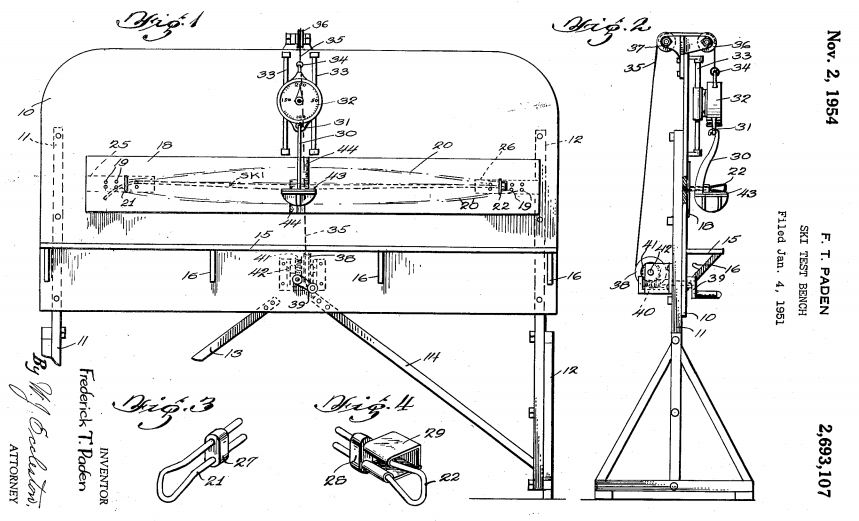
\includegraphics[width=1\textwidth]{figures/earlytb.png}
    \caption{Illustrating the concept of a test bench. Figure from \url{https://patents.google.com/patent/US2693107A/}}
    \label{fig:earlytb}
\end{figure}

The performance of a cross-country skier is highly dependent on the performance and quality of the skis. The ski's performance is determined by several mechanical properties such as the camber height and stiffness. These characteristics will be explained in detail later in this thesis. Another vital factor for the performance of the ski is the wax applied under the skis, both the grip wax to make the ski grip and the gliding wax to make the ski glide. However, it is often claimed that the performance of the skis themselves are roughly 80\% of the total performance, while the remaining approximately 20\% is influenced by the skier and service personnel \citep{ronbeck_vikander_2007,ronbeck_2001}. Grinding of the ski sole is roughly 10\% and the waxing also only 10\%. 

Finding the best skis is a challenge. Skis are chosen by the athletes and the experts together to find the best fit for the athlete. Great resources and time are being spent on manually selecting a large pool of skis for testing in the field. To the author's knowledge, the skis are hand-picked from the manufacturers by experts with intuition and experience. The skis are then stored in a pool of skis for further testing. The manual selection can indicate that the differences in each ski selected are prone to human error in terms of subjective selection. Furthermore, a quantitative way of choosing skis can further improve the ski selection phase by performing objective measurements and selection.

Older methods of testing mechanical properties in materials were done by applying force to the middle of a structure. A measurement device, shown in Figure \ref{fig:earlytb} was typically used to investigate the elasticity of structures like aircraft wings or skis. The concept was to apply forces to the center of the structure, to determine deflection or stress.
Companies like \textit{Skiselector} \ref{subsec:skiselector} and \textit{Gear West Signature Flex Tester} \ref{subsec:gwsft} have developed measurement devices with similar concepts, with focus on measuring the height of the camber and stiffness when applying an external force on the ski. By measuring and collecting mechanical properties, these measurement systems can give each ski a span curve profile used for matching similar skis.

\subsection{Body Weights and Loading Weights}
\label{subsec:bw}
When collecting mechanical properties during measuring of skis, it is necessary to load the ski with the correct weight for the matching ski-phase. These ski phases are the kick phase and the glide phase. Finding the gripping zone, and extracting mechanical properties, the weight of the skier is loaded. The full body weight (FBW) of the skier is loaded to find grip zones. For different snow conditions in terms of warm-, zero- or cold-weather $(\SI{2}{\celsius}> \SI{0}{\celsius} >\SI{-3}{\celsius})$,  the amount of contact from the grip zone during kick-phase is determined by the stiffness of the ski.
During the gliding phase, the skier balances the weight equally onto both skis to avoid the gripping wax from getting contact with the surface. For this phase, the weight loaded on the ski is defined to be the skiers half body weight (HBW).
These weights represent the loads applied on the ski for collecting the mechanical properties of the ski, during kick phase and gliding phase. The binding point (BP), is the point on the ski where the shoe tip attaches to the ski binding and is the reference point of where the force is applied, either at the binding point directly, offset towards or away from the heel point of the binding. Typically, during the kick-phase, the skier wants to apply all force at the binding point for increased contact on the surface. When investigating the skis quality and ability to glide, it is necessary to analyze the mechanical properties of the ski at the skiers half body weight.

\section{Mechanical properties}
\label{sec:mechanicalproperties}
A cross country ski has many mechanical properties. The mechanical properties also referred to as the characteristics, are essential when describing and measuring the quality of a ski. These details are the arch, stiffness, and how the weight distributes along the ski, where the latter is the pressure distribution. Choosing skis with mechanical properties matching the weather conditions is the most important way of finding the right skis. Felix Breitschädel published several papers on different aspects of how the gliding speeds and overall performance can be improved by using skis with different mechanical properties and sole structures.
Furthermore, his thesis leads to the development of a new low-cost inertial measurement unit(IMU)-based sensor to investigate camber height and heat maps where the ski presses on the surface. This measurement unit produced reasonable estimates to distinguish between good and bad skis. The mechanical properties used imaging of the sole to generate heat maps of the pressure areas \citep{breitschadel_technical_2014}. 
\newline

\subsection{Span curve}
\label{subsec:spancurve}
The span curve is the curvature of a ski profile that represents the camber height along the longitudinal length of the ski at HBW or FBW. As shown in Figure \ref{fig:spancurve}, the force is applied at the balance point. The span curve is extracted by pushing the ski down and measuring the height from the surface to the ski sole. The span curve is further used to determine the flex and stiffness of the ski and is essential for finding matching cross-country skis and is also related to camber height \ref{subsec:camberheight}.

\begin{figure}
    \centering
    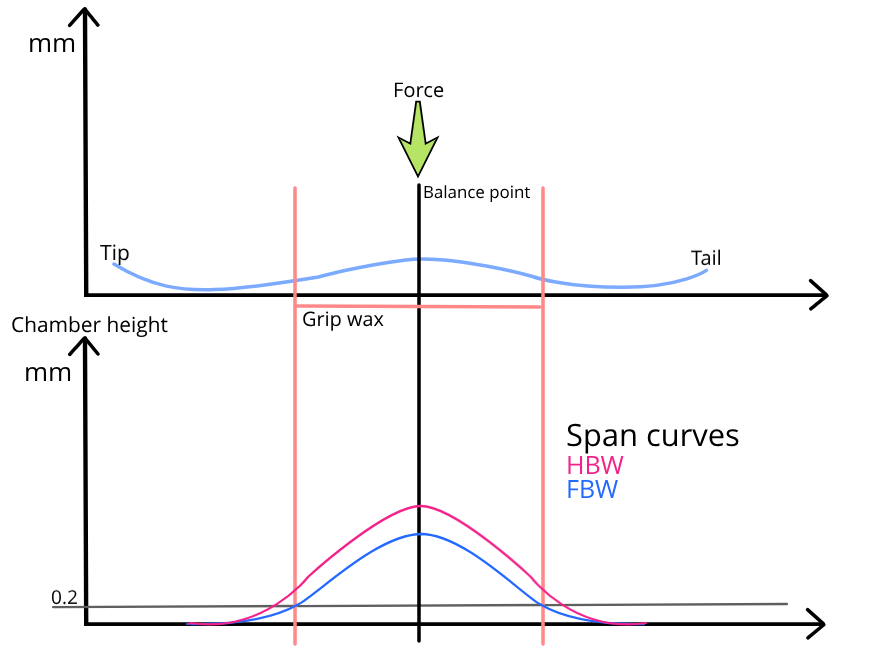
\includegraphics[width=1\textwidth]{figures/spancurve.png}
    \caption{An illustration of the span curves with HBW and FBW.}
    \label{fig:spancurve}
\end{figure}

\subsection{Camber height}
\label{subsec:camberheight}
The mechanical property camber height is described as the height from a flat surface to the sole of the ski.
The purpose of looking at the camber height at FBW and HBW is to find the contact area for gripping wax to be applied. Typically, the skis are marked on the side of the ski when the camber height is $0.2mm$ at both sides of the binding. Preferably, this height is when FBW is loaded. Contact is defined as the camber height at $0.05mm$ \citep{breitschadel_technical_2014}. Marking the waxing zone at FBW results in the gripping wax not establishing contact with the snow during the gliding phase (HBW).  The purpose of the marks is to define the gripping area on the sole, so the gripping wax establishes contact with the surface during kick phase  \citep{breitschadel_variation_2012}.
Furthermore, the definition of camber response is the change of camber height in $mm$ per $N$. The camber response is found by loading the BP from 0.5 to 1 times the BW. The camber response is used to calculate the stiffness of the ski \citep{breitschadel_technical_2014}.

\subsection{Stiffness}
\label{subsec:stiffness}
Stiffness is the skis ability to withold forces. Also, it is related to the stiffness at FBW and HBW when selecting a matching pair of skis. The purpose of this mechanical property is to estimate the stiffness of a ski when the body weights are loaded. Stiffness contributes to giving the wanted camber heights and span curve profiles for individual users concerning their body weight and is essential when finding a pair of matching skis for the different weather conditions. The stiffness, $k$, is the relation between the skier's body weight and the camber response of the ski.

\subsection{Pressure Distribution}
\label{subsec:pressuredistribution}
Pressure distribution is a mechanical property that describes the transferred forces to the surface along the longitudinal length of the cross-country ski. Pressure distribution characteristics are obtained by measuring the forces on the surface were the ski presses down. The purpose of measuring the forces at specific points is to find hot spots of forces on the surface which contributes to frictional melting (Section \ref{subsec:skisandsnow}), and how the ski structure distributes weight along the surface from the ski. Further on, fluctuation in the ski structure under stress indicates the ski quality in terms of twisting and even weight transfer along the latitudinal length of the ski. The pressure distribution can work as an additional property for finding a suited match of skis for an athlete. \cite{nilsson2013} researched how the force distribution changed when the loading point (center of mass) moved backward from the original BP position. This investigation can also confirm the interest of looking at the ski characteristics when a skier transitions from a kicking-phase to a gliding phase, where the skier shifts the body weight over to the heel in a resting position.

\begin{figure}
    \centering
    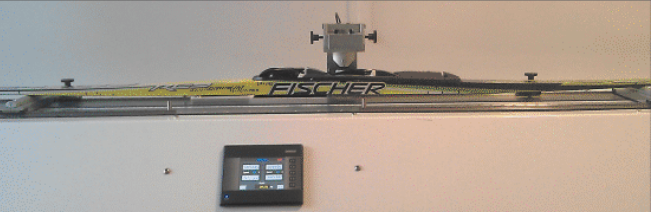
\includegraphics[width=1\textwidth]{figures/testbench.png}
    \caption{Ski test bench developed by Felix Breitschädel. Figure from \citep{breitschadel_technical_2014}}
    \label{fig:tbfelix}
\end{figure}

\section{What makes a ski glide?}
\label{sec:skiglide}
A ski gliding is when positive forces exceed the negative forces working on a skier (Section \ref{subsec:forces}). Positive gravity forces are generated either from going downhill or during kick-phase, resulting in gliding speeds. Overcoming the negative forces are essential for the performance of the skier. A ski slipping or gliding on the snow surface is dependant on the amount of friction between the ski sole and the surface. The friction determines the amount of frictional melting that occurs on the ski sole and generates a thin layer of water film, which decreases the friction. Snow and ice structures determine the amount of water film and friction that is needed. Different characteristics of the snow and snow crystals are not the aim of this study. Detailed characteristics on snow types and snow crystals were researched by \cite{ColbeckSC1986}, and is to the author's knowledge the most recognized and used classification scale for snow. Nevertheless, an understanding of how the forces are affecting the skier's total performance is necessary to investigate.

\subsection{Snow and Ice friction}
\label{subsec:skisandsnow}
Friction between a ski sole and snow or ice surface is highly dependant on; weather, temperature and snow conditions. Factors like the ski characteristics contribute to overcoming the negative forces and the delicate balance between friction and water film. A water film is a thin layer of water gathered up on the ski sole during skiing and is determined by the friction coefficient $\mu$ between the ski sole and the surface. This layer is a result of snow or ice melting due to frictional melting and works as lubrication for improved gliding speeds. The change in friction coefficient was already researched in the mid-nineteenth century by \citep{bowden1939mechanism}. They found that the friction coefficient decreased when the water film is introduced to the polyethylene sole surface \citep{bowden1939mechanism}.
Furthermore, a conclusion was derived that the friction was also related to temperature. Bowden and Hughes found that a decrease in temperature would increase the static friction, indicating lower friction in higher temperatures. 
When sliding speeds are noticeable, the friction decreases and approach a lower value with increasing speeds due to a localized surface melting produced by frictional melting \citep{bowden1953friction}.
A thicker water film is not always the best case for any weather condition. When the water film accumulated exceeds a threshold, and the water film generates drag, which results in reduced gliding speeds. 
More detailed research on the relation between the contact area with the surface and the water film thickness was conducted by \cite{baurle2006sliding}. The increased contact area with the surface with growing water film thickness is illustrated in Figure \ref{fig:waterfilm}. 
As friction is affected by the gravitational forces as well as the accumulated negative forces on the cross-country skier, it is in our best interest to investigate these for understanding which skis characteristics that contributes to better gliding speeds.
\begin{figure}[!htb]
     \centering
     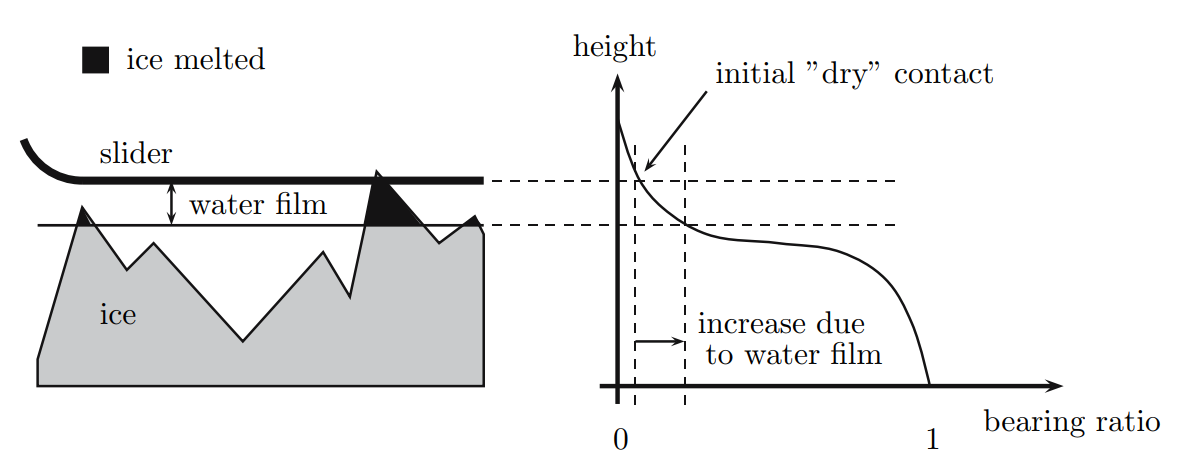
\includegraphics[width=0.99\textwidth]{figures/waterfilm.png}
     \caption{Relation between the water-film thickness and the real contact area (bearing ratio). Melting of ice corresponds to a slicing off and leads to the growth of existing contact and the formation of new contacts. Figure from \citep{baurle2006sliding}}
     \label{fig:waterfilm}
\end{figure}

\subsection{Forces working on the skier}
\label{subsec:forces}
In cross-country skiing, the forces illustrated in Figure \ref{fig:glidingforces} are propulsive forces generated through the skier's activity using a combination of poles and kicking and negative forces such as air resistance, drag, and friction. The objective of cross-country skiing is to overcome the negative forces affecting the skier. The forces acting on a skier in a gliding scenario is illustrated in Figure \ref{fig:glidingforces}. An explanation of the model was given thoroughly in \citep{breitschadel_technical_2014}.

According to Newton's \nth{2} Law, the forces in the direction of motion (x) are equal to the skier's mass, \textit{m}, times the acceleration, \textit{a}:
\begin{equation}\label{eqn:newtion2nd}
    \sum F_x = ma
\end{equation}

The skier's propulsion is affected by force ($F$) while gliding, which is the mass ($m$) times the gravity ($g$) on an inclined surface:
\begin{equation}
    F_D = F \sin\alpha = mg\sin\alpha
\end{equation}

The negative forces working against a skier's propulsive forces are air resistance ($F_{air}$) and, the frictional forces working between the snow or ice surface and the ski sole ($F_f$). The total sum of forces become:
\begin{equation}
    F_D - F_{air} - F_f = ma
\end{equation}

The friction coefficient ($\mu$) is defined as the resistance force ($F_f$) divided by the downward working force ($F_D$):
\begin{equation}\label{eqn:frictioneq}
    \mu = \frac{F_f}{F_N}
\end{equation}
\begin{figure}
    \centering
    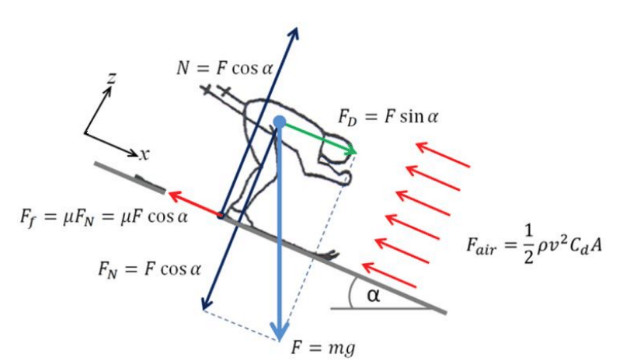
\includegraphics[width=1\textwidth]{figures/forces.png}
    \caption{The forces acting on a skier. Figure from \citep{breitschadel_technical_2014}}
    \label{fig:glidingforces}
\end{figure}
In relation to the pressure distribution \ref{subsec:pressuredistribution}, the static friction coefficient:
\begin{equation}\label{eqn:friction}
    F_{D} = F_f 
\end{equation}

\begin{equation*}\label{eqn:staticfriction}
    mg\sin\alpha = \mu_smg\cos\alpha
\end{equation*}

\begin{equation}\label{eqn:staticfriction2}
    \mu_s = \tan\alpha
\end{equation}
The static friction coefficient ($\mu_s$) is found when the ski is just about to slip ($F_D = F_f$). On the other hand, the kinetic friction coefficient ($\mu_k$) is of interest when the ski is gliding:
\begin{equation}\label{eqn:kineticfriction}
    F_D - F_f = ma
\end{equation}

\begin{equation*}
    mg\sin\alpha - \mu_kmg\cos\alpha = ma
\end{equation*}

\begin{equation*}
    \mu_k = \frac{g\sin\alpha}{g\cos\alpha} - \frac{a}{g\cos\alpha}
\end{equation*}

\begin{equation}\label{eqn:kineticfriction2}
    \mu_k = 
    \begin{cases}
    \mu_s       & \quad \text{if } a = 0\\
    \mu_s - \frac{a}{g\cos\alpha}  & \quad \text{if } a \neq 0
    \end{cases}
\end{equation}
\newline
The adjusting factor when applying the right gliding wax for warm-, zero- or cold-weather conditions, is the amount of kinetic friction between the snow or ice surface and the ski sole. Equation \ref{eqn:kineticfriction2} denotes that the kinetic friction coefficient is equal to the static friction coefficient when the acceleration is zero. At zero acceleration, the skier is in a gliding phase. The gliding wax can either reduce or increase the kinetic friction coefficient to give enough water film for better gliding speeds. For lower temperatures, one will see gliding wax which introduces higher $\mu_k$ for more frictional melting.

\section{Measurement devices}
\label{sec:measurementdevices}
The span curve is an essential descriptor of the mechanical properties of the ski. Several measurement devices have been developed to efficiently and accurately measure the span curve and camber height. The following sections investigate previous research on measurement devices with existing methods for extracting mechanical properties.

\subsection{Eiker måler}
\label{subsec:eiker}
The Eiker ski measurement device was initially developed for the winter Olympics in Lillehammer in 1994 by a Norwegian company called Ski-Test. The idea behind the Eiker-måler was to pair skis with similar flex, also referred to as span curve, and to find a reasonable match to the skier concerning stiffness to weight ratio. Since the start of Ski-test, they have been developing their system with great success, expanding the use to several countries, such as Sweden, Estland, Canada, and the USA to mention a few \citep{eiker_2018}. As instructed by the company, the electrical measurement device loads the ski with a skiers weight to HBW and FBW to mark the gliding zones and kicking zones for application of gliding wax and gripping wax respectively (Figure \ref{fig:eikermåler}).

\begin{figure}
    \centering
    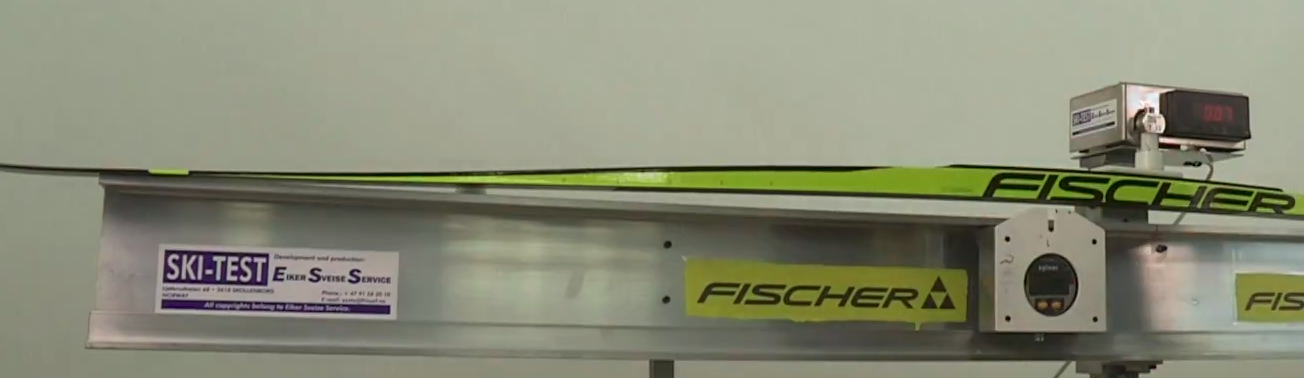
\includegraphics[width=1\textwidth]{figures/eiker.png}
    \caption{An illustration of the "Eiker-måler". Figure from \url{http://www.ski-test.no/instructions/}}
    \label{fig:eikermåler}
\end{figure}

\subsection{SkiSelector}
\label{subsec:skiselector}
The first SkiSelector system was developed for the winter Olympics in Turin in 2006. SkiSelector is a Swedish company, and have increased in popularity since 2006, founded in 2011, the SkiSelector Academy further development of the system. The system delivers a good overview of skis mechanical properties such as grip, stiffness, camber characteristics, and sliding properties. The goal of this system is to give the skier detailed information about the pair of skis and how the skis should be waxed for better grip and glide \citep{skiselector_2018}. The system looks similar to the "Eiker-måler" but instead uses a computer with software to create a profile of each ski measured.

\subsection{IDT Sport - SkiAnalyzer}
\label{subsec:idt}
The SkiAnalyzer from IDT Sport delivers a complete measurement system with different software versions matching the user's experience. The measurements are based on laser technology to measure the camber height and stiffness. Through the software, the system outputs span and stiffness curves. Furthermore, at the end of a measurement, the user can save the measurement data to a database for later use \citep{idt_2018}. The information given by IDT Sport on the SkiAnalyzer (Figure \ref{fig:skianalyzer}) is limited; the system seems to operate with the same precision as SkiSelector and Eiker Måler.

\begin{figure}
    \centering
    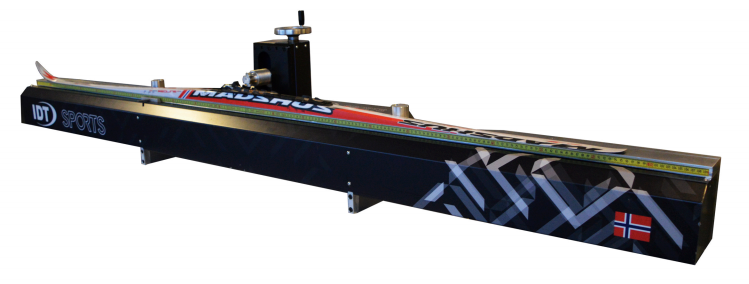
\includegraphics[width=1\textwidth]{figures/skianalyzer.png}
    \caption{An illustration of the SkiAnalyzer from IDT Sport. Figure from \url{https://www.idt.no/sport/produkter/skianalyzer/skianalyzer}}
    \label{fig:skianalyzer}
\end{figure}

\subsection{Gear West Signature Flex Tester}
\label{subsec:gwsft}
Gear West developed the system Ski DNA \citep{skidna_2018}. The system consists of three phases for choosing and measuring cross-country skis, where the first phase is using hands and eyes when squeezing the skis. After the subjective selection, the skier will apply body weight in different positions on the ski. By loading the ski, the ski pocket is found to ensure that the selected skis match each other. The third phase is to put the skis through the Flex Tester measurement bench. The measurement bench is designed to use loading cells to collect pressure distribution data. This data allows the system to check the quality of the flex, weight range, and ideal snow condition for the skis.

\section{Chapter discussion}
In 2008, Bäckström investigated mechanical properties, such as span curve and pressure distribution, and the importance of finding the pressure distribution was further confirmed by Erkillä (1986). These mechanical properties are factors that are affecting the friction, $\mu$, between the skis and snow. Ekström (1980) showed that the friction, $\mu$, decreases with an increased camber value.


\section{Chapter summary}
\label{sec:backgroundconclusion}
Mechanical properties will always be a defining factor between a winning and losing pair of skis. Selecting the right ski for different weather conditions has a significant role in the ski selection phase. A stiffer ski with a short nominal running surface is typically found in classical cross-country skis for warm-weather conditions, giving a steeper increase in camber height at the start of the wax pocket. Warm-weather conditions require a stickier grip wax which introduces a thicker layer of wax. The steep increase in camber height decreases the probability of the gripping wax in the wax pocket and reducing the chance of getting contact with the surface during a gliding phase.
On the contrary, a ski with a more extended nominal running surface is found on classical cross-country skis for cold weather condition. The gripping wax has a dryer consistency, which reduces the overall height of gripping wax applied. The extended nominal contact area will also introduce more frictional melting for generating more water film for better gliding speeds in colder weather conditions.

Based on how the athlete's body weight is loaded on the ski, by for example different pressure points of the foot, varying results in pressure zones onto the ice or snow surface occurs. The thought is that a stiffer structure on the inside of a ski can be countered by a matching weight profile of the foot with extended pressure on the inner side of the foot, resulting in an overall flatter contact of the latitudinal running surface of a ski. With this in mind, it is possible that the friction is more evenly distributed on the surface, resulting in more consistent heat generation and water film due to frictional melting of ice or snow.

The Ski DNA system (Section \ref{subsec:gwsft}), is by far the most interesting. More specifically, the use of loading cells to measure pressure distribution. By using loading cells on prefixed location along with the longitudinal running surface of the ski, we can investigate the forces on each of these points. This investigation could result in pressure distribution profiles for assisting in ski selection. Breitschädel explained that a measurement uncertainty with the Ski Analyzer (Section \ref{subsec:idt}), was affected by the ski running surface. Some sensors on the system could not register contact with the ski, due to the twisting in the skis material.
To the author's knowledge, twisting in the ski structures is a result of deformation of the materials in the ski under production. Finding skis with minimal twisting can result in a more evenly distribution of weight onto ice or snow surface. Twisting can also be considered a property of interest to match the weight transfer from a foot to the ski.
The lack of knowledge on twisting and pressure distribution profiles on classical cross-country skis motivates the development of a measurement device to register both. A measurement device is researched and designed to investigate mechanical properties in classical cross-country skis. In the following sections, a further expansion on existing research and designs lead by multiple sources, such as \cite{ronbeck_2001}, \cite{breitschadel_variation_2012,breitschadel_technical_2014} is further developed.

